\documentclass[10pt]{beamer}

\usepackage{packages}
\title{Exercício Programa 1}
\subtitle{Escalonador de processos}
\institute{IME-USP}
\author{Lucas Paiolla Forastiere e Marcos Siolin Martins}
\date{05 de outubro de 2020}

\begin{document}
    \maketitle
    \section{Shell}
    \begin{frame}{Arquitetura do Shell}
    \end{frame}

    \section{Escalonadores}
    \subsection{Implementação}
    \begin{frame}{Implementação dos Escalonadores}
    \end{frame}

    \subsection{Experimentos}
    \begin{frame}{Arquivo de Trace: 10 processos}
        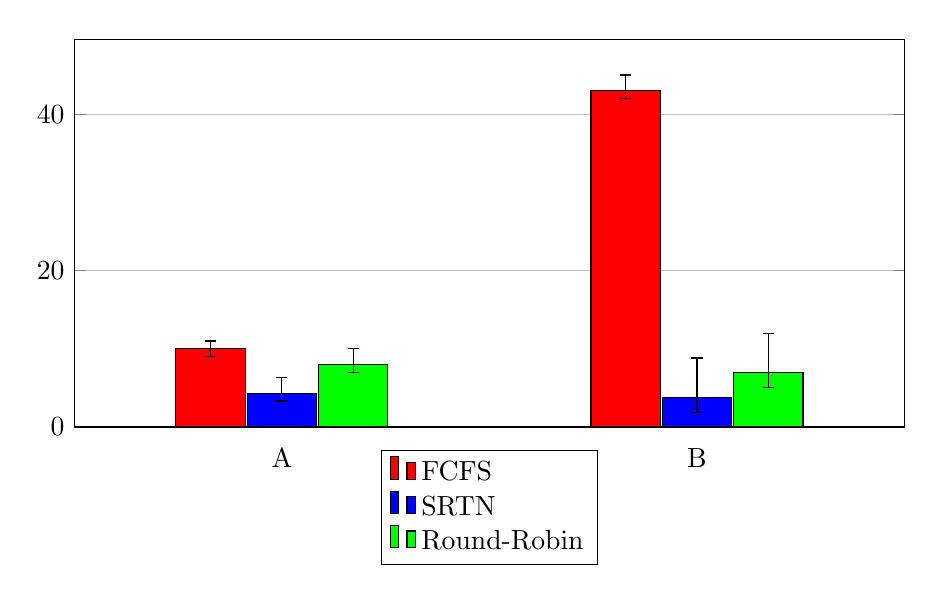
\begin{tikzpicture}
              \begin{axis}[
                  width  = 1.00*\textwidth,
                  height = 6.5cm,
                  major x tick style = transparent,
                  ybar=2*\pgflinewidth,
                  bar width=25pt,
                  ymajorgrids = true,
                  symbolic x coords={A,B},
                  xtick = data,
                  scaled y ticks = false,
                  enlarge x limits=0.50,
                  ymin=0,
                  legend cell align=left,
                  legend style={at={(0.5,-0.06)},anchor=north},
              ]

              \addplot[style={fill=red},
                error bars/.cd,
                y dir=both,
                y explicit]
              coordinates {
                  (A, 10) += (0,1) -= (0,1)
                  (B, 43) += (0,2) -= (0,1)
              };

              \addplot[style={fill=blue},
                error bars/.cd,
                y dir=both,
                y explicit]
              coordinates {
                   (A,4.33) += (0,2) -= (0,1)
                   (B,3.82) += (0,5) -= (0,2)
              };

              \addplot[style={fill=green},
                error bars/.cd,
                y dir=both,
                y explicit]
              coordinates {
                   (A,8) += (0,2) -= (0,1)
                   (B,7) += (0,5) -= (0,2)
              };


              \legend{FCFS, SRTN, Round-Robin}
            \end{axis}
        \end{tikzpicture}
    \end{frame}

    \begin{frame}{Arquivo de Trace: 100 processos}
        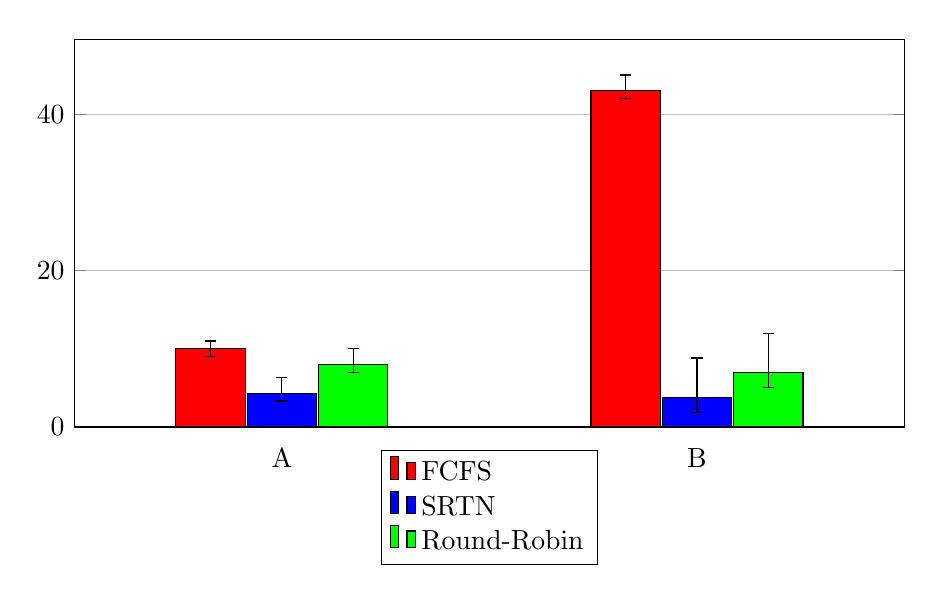
\begin{tikzpicture}
              \begin{axis}[
                  width  = 1.00*\textwidth,
                  height = 6.5cm,
                  major x tick style = transparent,
                  ybar=2*\pgflinewidth,
                  bar width=25pt,
                  ymajorgrids = true,
                  symbolic x coords={A,B},
                  xtick = data,
                  scaled y ticks = false,
                  enlarge x limits=0.50,
                  ymin=0,
                  legend cell align=left,
                  legend style={at={(0.5,-0.06)},anchor=north},
              ]

              \addplot[style={fill=red},
                error bars/.cd,
                y dir=both,
                y explicit]
              coordinates {
                  (A, 10) += (0,1) -= (0,1)
                  (B, 43) += (0,2) -= (0,1)
              };

              \addplot[style={fill=blue},
                error bars/.cd,
                y dir=both,
                y explicit]
              coordinates {
                   (A,4.33) += (0,2) -= (0,1)
                   (B,3.82) += (0,5) -= (0,2)
              };

              \addplot[style={fill=green},
                error bars/.cd,
                y dir=both,
                y explicit]
              coordinates {
                   (A,8) += (0,2) -= (0,1)
                   (B,7) += (0,5) -= (0,2)
              };


              \legend{FCFS, SRTN, Round-Robin}
            \end{axis}
        \end{tikzpicture}
    \end{frame}

    \begin{frame}{Arquivo de Trace: 1000 processos}
        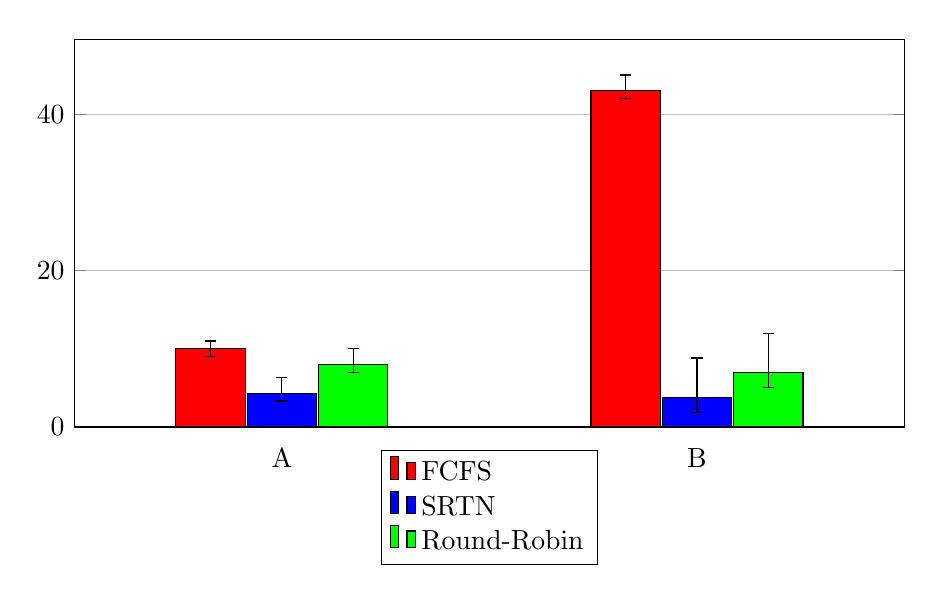
\begin{tikzpicture}
              \begin{axis}[
                  width  = 1.00*\textwidth,
                  height = 6.5cm,
                  major x tick style = transparent,
                  ybar=2*\pgflinewidth,
                  bar width=25pt,
                  ymajorgrids = true,
                  symbolic x coords={A,B},
                  xtick = data,
                  scaled y ticks = false,
                  enlarge x limits=0.50,
                  ymin=0,
                  legend cell align=left,
                  legend style={at={(0.5,-0.06)},anchor=north},
              ]

              \addplot[style={fill=red},
                error bars/.cd,
                y dir=both,
                y explicit]
              coordinates {
                  (A, 10) += (0,1) -= (0,1)
                  (B, 43) += (0,2) -= (0,1)
              };

              \addplot[style={fill=blue},
                error bars/.cd,
                y dir=both,
                y explicit]
              coordinates {
                   (A,4.33) += (0,2) -= (0,1)
                   (B,3.82) += (0,5) -= (0,2)
              };

              \addplot[style={fill=green},
                error bars/.cd,
                y dir=both,
                y explicit]
              coordinates {
                   (A,8) += (0,2) -= (0,1)
                   (B,7) += (0,5) -= (0,2)
              };


              \legend{FCFS, SRTN, Round-Robin}
            \end{axis}
        \end{tikzpicture}
    \end{frame}

    \begin{frame}{Conclusões dos experimentos}
        \begin{enumerate}
        \end{enumerate}
    \end{frame}

\end{document}
